\documentclass[10pt, xcolor = svgnames]{beamer} %Beamer
\usepackage{palatino} %font type
\usefonttheme{metropolis} %Type of slides
\usefonttheme[onlymath]{serif} %font type Mathematical expressions
\usetheme[progressbar = frametitle,titleformat frame=smallcaps,numbering=counter]{metropolis} %This adds a bar at the beginning of each section.
\useoutertheme[subsection=false]{miniframes} %Circles in the top of each frame, showing the slide of each section you are at

\usepackage{appendixnumberbeamer} %enumerate each slide without counting the appendix
\setbeamercolor{progress bar}{fg=Maroon!70!Coral} %These are the colours of the progress bar. Notice that the names used are the svgnames
\setbeamercolor{title separator}{fg=DarkSalmon} %This is the line colour in the title slide
\setbeamercolor{structure}{fg=black} %Colour of the text of structure, numbers, items, blah. Not the big text.
\setbeamercolor{normal text}{fg=black!87} %Colour of normal text
\setbeamercolor{alerted text}{fg=DarkRed!60!Gainsboro} %Color of the alert box
\setbeamercolor{example text}{fg=Maroon!70!Coral} %Colour of the Example block text


\setbeamercolor{palette primary}{bg=NavyBlue!50!DarkOliveGreen, fg=white} %These are the colours of the background. Being this the main combination and so one. 
\setbeamercolor{palette secondary}{bg=NavyBlue!50!DarkOliveGreen, fg=white}
\setbeamercolor{palette tertiary}{bg=NavyBlue!40!Black, fg= white}
\setbeamercolor{section in toc}{fg=NavyBlue!40!Black} %Color of the text in the table of contents (toc)

%These next packages are the useful for Physics in general, you can add the extras here. 
\usepackage{amsmath, amssymb}
\usepackage{slashed}
\usepackage{cite}
\usepackage{relsize}
\usepackage{caption}
\usepackage{subcaption}
\usepackage{multicol}
\usepackage{booktabs}
\usepackage[scale=2]{ccicons}
\usepackage{pgfplots}
\usepgfplotslibrary{dateplot}
\usepackage{geometry}
\usepackage{xspace}
\usepackage[useregional]{datetime2}
\newcommand{\themename}{\textbf{\textsc{bluetemp}\xspace}}%metropolis}}\xspace}
\newcommand{\cald}{{\rm d}}

\newcommand{\TEX}[0]{~
\includegraphics[height = 9.5pt]{./logos/TeX.pdf}}
\newcommand{\LATEX}[0]{~\includegraphics[height = 9.5pt]{./logos/LATeX.pdf}}
\newcommand{\FORTRAN}[0]{~
\includegraphics[height = 9.5pt]{./logos/Fortran.pdf}}
\newcommand{\PYTHON}[0]{~
\includegraphics[height = 9.5pt]{./logos/Python.pdf}}
\newcommand{\MMA}[0]{~
\includegraphics[height = 9.5pt]{./logos/Mathematica.pdf}}
\newcommand{\CERN}[0]{~
\includegraphics[height = 9.5pt]{./logos/CERN_ROOT.pdf}}
\newcommand{\GPT}[0]{~
\includegraphics[height = 9.5pt]{./logos/GPT.pdf}}
\newcommand{\ALL}[0]{\FORTRAN\PYTHON\MMA}
\newcommand\blfootnote[1]{
  \begingroup
  \renewcommand\thefootnote{}\footnote{#1}
  \addtocounter{footnote}{-1}
  \endgroup
}



\usepackage{listings}
\usepackage{color}
\usepackage{bigints}

\definecolor{dkgreen}{rgb}{0,0.6,0}
\definecolor{gray}{rgb}{0.5,0.5,0.5}
\definecolor{mauve}{rgb}{0.58,0,0.82}

\lstset{frame=tb,
  language=FORTRAN,
  aboveskip=3mm,
  belowskip=3mm,
  showstringspaces=false,
  columns=flexible,
  basicstyle={\small\ttfamily},
  numbers=none,
  numberstyle=\tiny\color{gray},
  keywordstyle=\color{blue},
  commentstyle=\color{dkgreen},
  stringstyle=\color{mauve},
  breaklines=true,
  breakatwhitespace=true,
  tabsize=4
}






\title{Computer Programming \\ on Geosciences}
%\author[Name]{Gauss \textsc{Chang}\inst{$\dagger$}, others\inst{$\ddagger$} and supervisor's name\inst{$\ast$}} %With inst, you can change the institution they belong
\author[Name]{Gauss \textsc{Chang}\inst{$\dagger$}} %With inst, you can change the institution they belong
\subtitle{Numerical Integration Methods}


\institute[uni] % (optional)
{
	\inst{\dagger}
	Department of Physics \\
	\textsc{National Taiwan University}
%	\and
%	\inst{\ddagger}
%	Department of Something \\
%	\textsc{others' Institute}
%	\and
%	\inst{\ast}
%	Department of Something \\
%	\textsc{Supervisor's Institute}
}


% \date{\today} %Here you can change the date
\date{\DTMdate{2024-09-18}} %Here you can change the date

\titlegraphic{\vspace{0.0cm}\hfill
\includegraphics[width = 0.25\textwidth]{./logos/NTU.pdf}}

\begin{document}
{
\setbeamercolor{background canvas}{bg=NavyBlue!50!DarkOliveGreen, fg=white}
\setbeamercolor{normal text}{fg=white}
\maketitle
}%This is the colour of the first slide. bg= background and fg=foreground

\metroset{titleformat frame=smallcaps} %This changes the titles for small caps




\begin{frame}{Outline}
  \setbeamertemplate{section in toc}[sections numbered] %This is numbering the sections
  \tableofcontents[hideallsubsections] %You can comment this line if you want to show the subsections in the table of contents
\end{frame}




%\begin{frame}{Objectives}
%\underline{\textsc{Some text:}}
%\begin{small}
%This is some small Text. 
%\end{small}
%
%\metroset{block=fill}
%\begin{exampleblock}{\textsc{Example block}}
%\begin{itemize}
%    \item You know how to do itemize
%    \item Also here
%\end{itemize}
%\end{exampleblock}
%\end{frame}



\section{Inspiration}

\begin{frame}[fragile]{Inspiration: An Interesting Question}
I saw this interesting question a few month ago:

\metroset{block=fill}
\begin{exampleblock}{\textsc{Question}}
How do you prove that
\begin{align}
	\pi^3
	&> 31
\end{align}
\end{exampleblock}
\blfootnote{\ALL}
\end{frame}

\begin{frame}[fragile]{Inspiration: An Interesting Question}
And there was a brilliant answer:

\metroset{block=fill}
\begin{exampleblock}{\textsc{Proof}}
Notice that
\begin{align}
	\bigints_0^1 \left[ \frac{8 x^5 \left( 1 - x \right)^2 \left( 324889 - 120736 x^2 \right) }{445625 \left( 1 + x^2 \right) } \cdot \left( \ln^2 x \right) \right] \,\cald x
	% \int_0^1 \frac{8 x^5 \left( 1 - x \right)^2 \left( 324889 - 120736 x^2 \right) }{445625 \left( 1 + x^2 \right) } \cdot \left( \ln^2 x \right) dx
	&= \pi^3 - 31
\end{align}

since the integrand is positive over the region, the integral is also positive.

Trivially, $\pi^3 > 31$ is proven.
\end{exampleblock}
\end{frame}



\section{Addressing The Problem}

\begin{frame}[fragile]{Addressing The Problem: Construct Function}


Here is an example code for the integrand.
\begin{lstlisting}
function integrand(x) result(res)
    implicit none
    real :: x
    real :: numerator, denominator, res
    real, parameter :: C1 = 324889.0
    real, parameter :: C2 = 120736.0
    real, parameter :: C3 = 445625.0
    numerator = 8.0 * x**5 * (1.0 - x)**2 * (C1 - C2 * x**2) * (log(x))**2
    denominator = C3 * (1.0 + x**2)
    res = numerator / denominator
end function integrand
\end{lstlisting}
\blfootnote{\FORTRAN}
\end{frame}

\begin{frame}[fragile]{Addressing The Problem: Plot The Integrand}

Try to plot the integrand, just make sure it is a ``well-behaved'' function.

\begin{figure}
\centering
\includegraphics[width=0.5\textwidth]{./plot/Integrand_FORTRAN.pdf}
\caption{$\frac{8 x^5 \left( 1 - x \right)^2 \left( 324889 - 120736 x^2 \right) }{445625 \left( 1 + x^2 \right) } \cdot \left( \ln^2 x \right)$}
\label{plot1}
\end{figure}
\blfootnote{\FORTRAN}
\end{frame}




\section{Approach One}








\begin{frame}[fragile]{Approach One: Monte Carlo Method}


Here is an example code for the integrand.
\lstset{language=Python}
\begin{lstlisting}
def integrand(x: float) -> float:
    C1: Final = 324889
    C2: Final = 120736
    C3: Final = 445625

    numerator = 8 * x**5 * (1 - x)**2 * (C1 - C2 * x**2) * (np.log(x))**2
    denominator = C3 * (1 + x**2)

    return numerator / denominator
\end{lstlisting}
\blfootnote{\PYTHON}
\lstset{language=FORTRAN}
\end{frame}


\begin{frame}[fragile]{Approach One: Monte Carlo Method}


Here is another example code for the integrand.
\lstset{language=C++}
\begin{lstlisting}
double integrand(double x) {
    const double C1 = 324889;
    const double C2 = 120736;
    const double C3 = 445625;
	
    double numerator = 8 * pow(x, 5) * pow(1 - x, 2) * (C1 - C2 * pow(x, 2)) * pow(log(x), 2);
    double denominator = C3 * (1 + pow(x, 2));
    
    return numerator / denominator;
}
\end{lstlisting}
\blfootnote{\CERN}
\lstset{language=FORTRAN}
\end{frame}








\begin{frame}[fragile]{Fortran Basic: Fortran is formatted}

\begin{minipage}{0.45\textwidth}
Fortran 77
\begin{itemize}
	\item Fixed Format
	\item 1-72 char
\end{itemize}
\begin{lstlisting}
Program Test
declare
...
Stop
End
\end{lstlisting}
\end{minipage}
\hspace{20pt}
\begin{minipage}{0.45\textwidth}
Fortran 90
\begin{itemize}
	\item Free Format
	\item 1-132 char
\end{itemize}
\begin{lstlisting}
Program test
declare
...
End program test
\end{lstlisting}
\end{minipage}
\end{frame}

\begin{frame}[fragile]{Fortran Basic: Fixed Format}
``Fixed Format'' regulates different roles of character positions. Columns 7-72 are used for coding. The first 5 columns can only be blank or contain a numeric label. Column 6 can only be a nonblank, nonzero character to be identified as a  continuation line.
%\begin{table}[]
%\begin{tabular}{|l|l|}
%\hline
%Column(s) & Illustration                                                                              \\ \hline
%1         & If it is ‘C’, ‘c’, or ‘*’, this line will be treated as comment and not be compiled.      \\ \hline
%1-5       & If a number is put here, it is the lable of the line. Otherwise, it can only be blank.    \\ \hline
%6         & Except zero or blank, any character here indicates that this line is a continuation line. \\ \hline
%7-72      & Coding region.                                                                            \\ \hline
%after 73  & Not using. Anything here will be omitted. Some compilers could report error message.      \\ \hline
%\end{tabular}
%\end{table}
\end{frame}



%\begin{frame}[fragile]{Introduction: blah blah} %You can change fragile by standout
%Text Text Text Text. \\You can change the size of the footnote text like  Text\footnote{\small{ here.}} Text\footnote{\large{And here.}} Text\footnote{\tiny{And here.}}
%\begin{itemize} %The symbol of the items can be changed by which ever you want, this is just an example.
%    \item[$\diamond$] Text,
%    \item[$\diamond$] Text,
%    \item[$\diamond$] Text.
%\end{itemize}
%An equation without number could be represented by:
%\begin{equation*}
%    c^{2} = a^{2} + b^{2}
%\end{equation*}
%That's all for this slide.
%\end{frame}


%\begin{frame}[standout]{This is other type of slide}
%There is some text here.
%And an equation with number:
%\begin{equation}
%    E^{2} = m^{2} + p^{2}
%\end{equation}
%\end{frame}


%\begin{frame}{Include a Figure}
%\begin{small}
%Something about the fig.
%\end{small}
%\begin{figure}
%\centering
%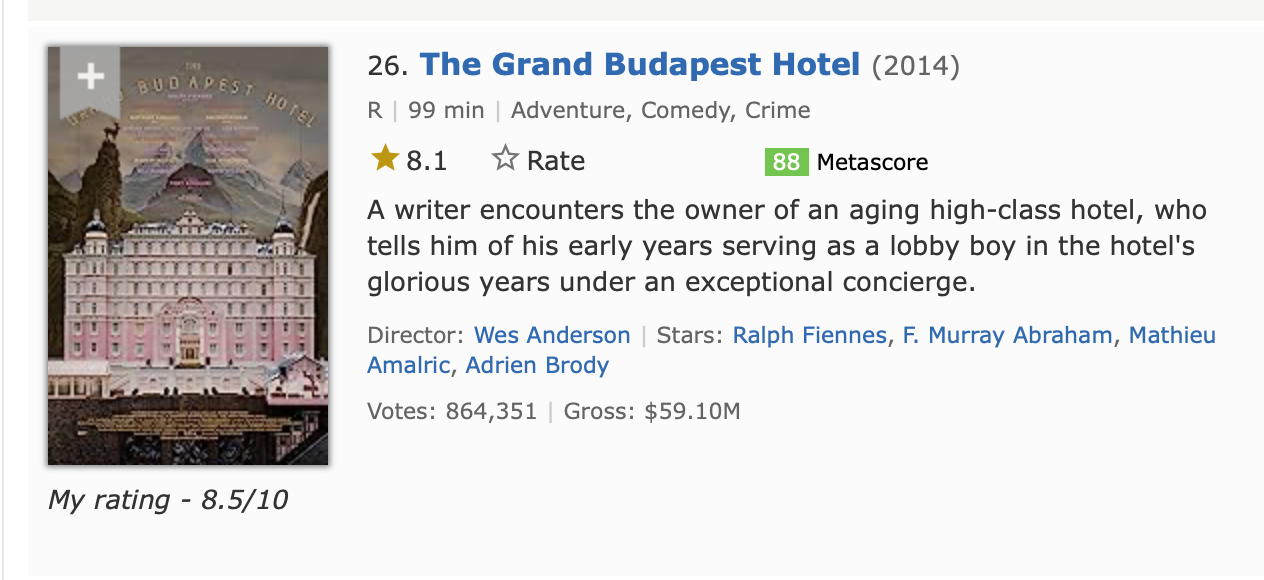
\includegraphics[width=0.7\textwidth]{./fig/fig1}
%\caption{Screenshot from the IMDb website.}
%\label{fig1}
%\end{figure}
%\end{frame}


%\begin{frame}[fragile]{Another way to include a Figure}
%\begin{minipage}{0.45\textwidth}
%\begin{enumerate}
%	\item Released in 2014
%	\item A comedy-drama
%	\item Directed by Wes Anderson
%\end{enumerate}
%\end{minipage}
%\hspace{20pt}
%\begin{minipage}{0.45\textwidth}
%\begin{figure}
%\centering
%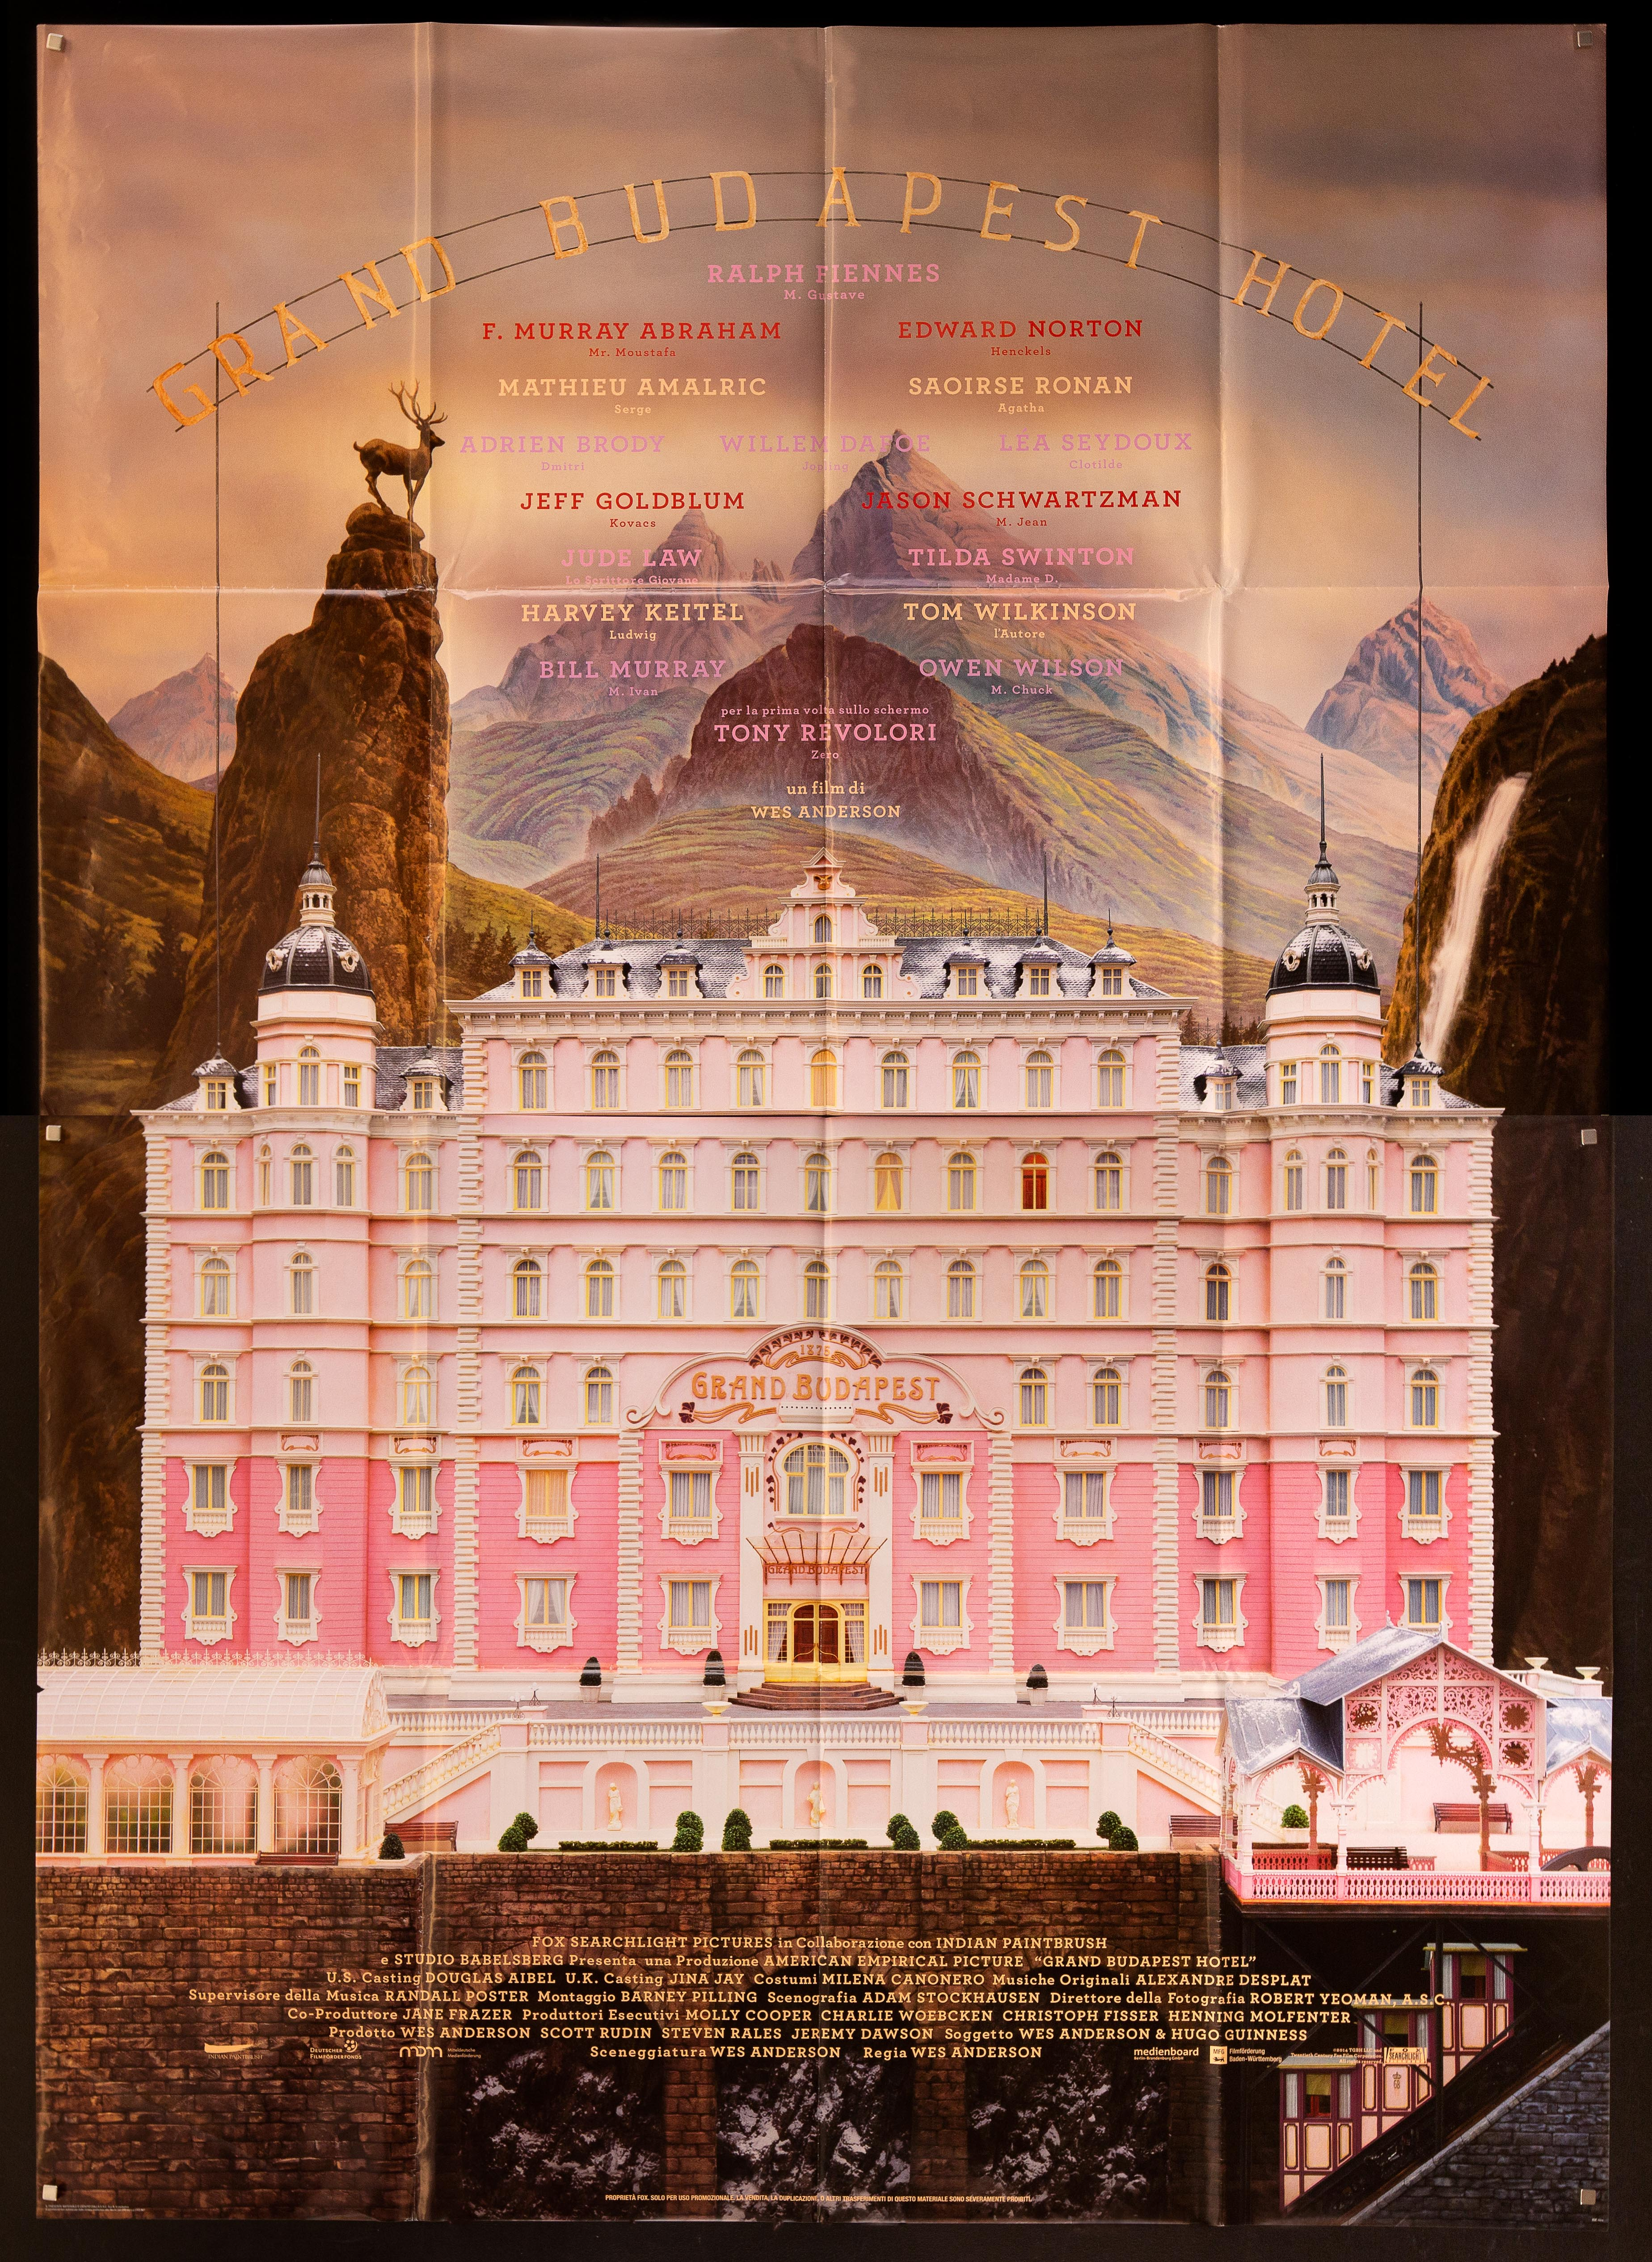
\includegraphics[width = 0.8\textwidth]{./fig/poster.jpg}
%\caption{Poster.}
%\label{fig1}
%\end{figure}
%\end{minipage}
%\end{frame}



%\section{Final section}
%
%\begin{frame}{Conclusion}
%    These are the final words, you do your best to try to wake up everyone that was listening to your talk.
%\end{frame}


%{\setbeamercolor{palette primary}{fg=black, bg=orange!30} %You can change the colours
%\begin{frame}[standout]
%  Thank you! And thank to yourself because you did all the job. 
%\end{frame}
%}

%\section{Bibliography}
%
%\begin{frame}[allowframebreaks]{Bibliography}
%\nocite{*}
%\bibliographystyle{unsrt}
%\bibliography{./bibliography.bib}
%\end{frame}


\end{document}












